\newSec[Quads]{\Quad\ als System}{1}





\newSec{Orientierungsmerkmale}{2}




\begin{figure}[ht!]
\vspace{0.25cm}
\begin{center}
\fbox{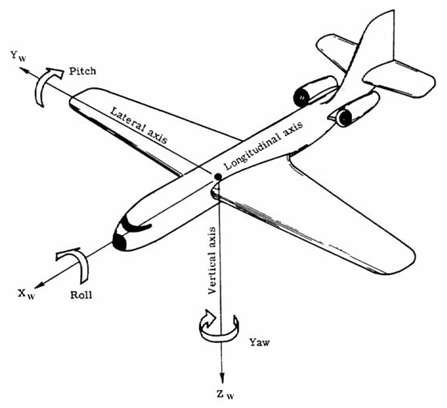
\includegraphics[width=12cm]{Pictures/Orientations.png}}
\caption{Orientierungsmerkmale eines Flugobjekts \cite{parotSDK}}
\label{fig:Orient}
\end{center}

\vspace{0.25cm}
\refImgShort{fig:Orient} zeigt die Orientierung eines beliebigen Flugobjektes am beispiel eines Flugzeugs. Die Bezeichner beziehen sich auf ein kartesisches Korrdinatensystem und beschrieben jeweils die Rotation um eine Raumachse.
\end{figure}






\newSec{Geometrien}{2}
Bei \Quad[n] handelt es sich um Fluggeräte mit vier Rotoren, welche horizontal angebracht sind. Der Auftrieb wird somit unmittelbar durch die Rotoren induziert.

Das Drehmoment der Rotoren des \Quad[s] muss sich aufheben können, um eine unkontrollierbare Rotation um die z-Achse vermeiden zu können. Um die Agilität des \Quad[s] beibehalten zu können, sind die Drehrichtungen der Rotoren zu alternieren.\comp{Paper1} \refImg{fig:Forces} deutet die Kräfte und aus der Rotationsgeschwindigkeit der Rotoren ableitbare Momente eines \Quad[s] an. Dies soll als Einleitung für das \refCap{Freiheitsgrade} dienen und wird an dieser Stelle nicht näher vertieft.

\begin{figure}[ht!]
\vspace{0.25cm}
\begin{center}
\fbox{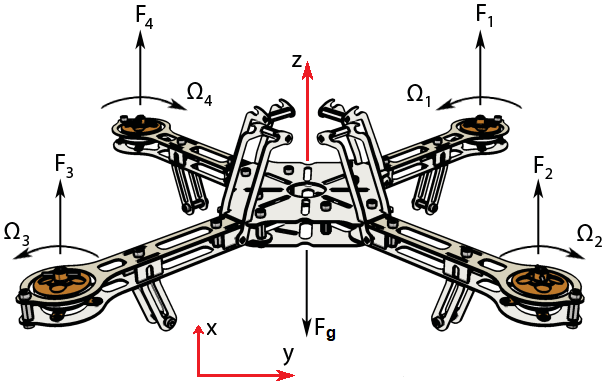
\includegraphics[width=12cm]{Pictures/Forces.png}}
\caption{wirkende Kräfte am \Quad\ in \textbf{x}-Anordnung \comp{Paper2}}
\label{fig:Forces}
\end{center}

\vspace{0.25cm}
\refImgShort{fig:Forces} zeigt die wirkenden Kräfte an einem \Quad\ in \textbf{x}-Anordnung. Die Achsen das Koordinatensystems sind in \textcolor{red}{rot} markiert. Alle mit \textit{F} markeirten Pfeile deuten Kräfte an. Die mit $\Omega$ markierten gebogenen Pfeile zeigen die Rotationsgeschwindigkeit der einzelnen Rotoren.
\end{figure}


Die Rotoren von \Quad[n] können in zwei verschiedenen Anordnungen angebracht werden (siehe \refImg{fig:Geom}).

\begin{figure}[ht!]
\vspace{0.25cm}
\begin{center}
\fbox{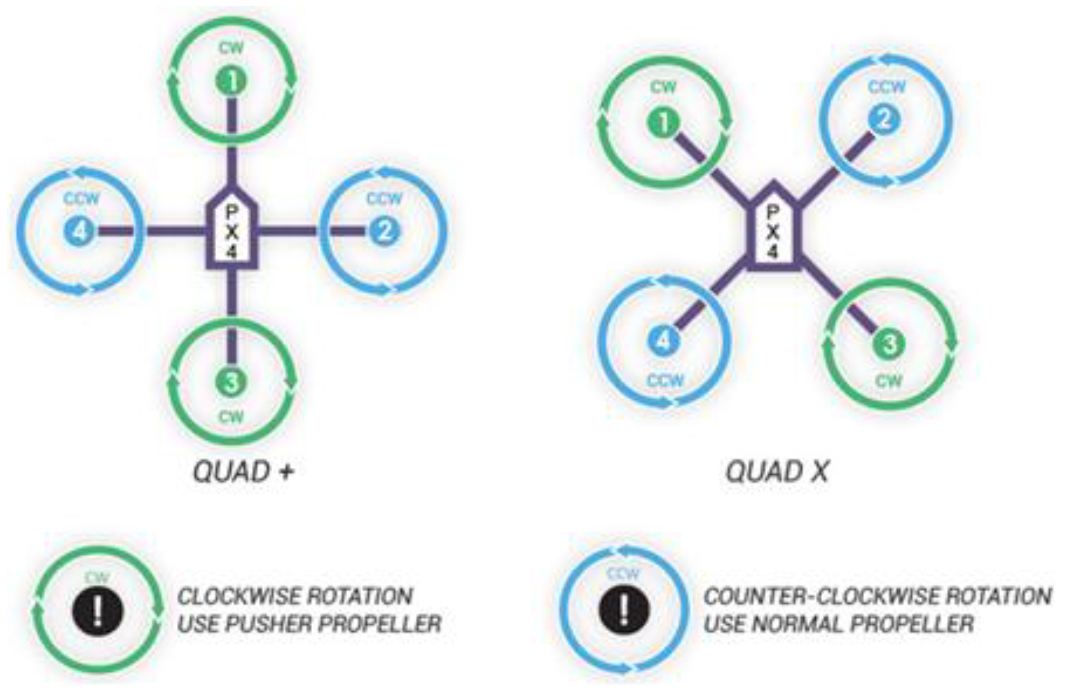
\includegraphics[width=12cm]{Pictures/Geometries.png}}
\caption{Geometrien von \Quad[n] \cite{Paper1}}
\label{fig:Geom}
\end{center}

\vspace{0.25cm}
\end{figure}


\newSec[Plus]{\textbf{+}-Anordnung}{4}
In der \textbf{+}-Anordnung befinden sich die Rotoren auf den Objekt-Achsen des \Quad[s]. Die Nummerierung der Rotoren erfolgt gemäß \refImg{fig:Geom} (links) im Uhrzeigersinn beginnend mit dem Rotor auf der positiven x-Achse.


\newSec[X]{\textbf{x}-Anordnung}{4}
Die \textbf{x}-Anordnung scheint nach online Recherchen weiter verbreitet. Eine mögliche Begründung findet sich in der weniger verdeckten Sicht für Frontkameras oder andere Anbaugeräte.



\newSec{Freiheitsgrade}{2}
Einem \Quad\ können sechs Freiheitsgrade zugewiesen werden, jeweils drei der Position und der Orientierung im Raum.\\
Nachfolgend wird physikalisch begründet, weshalb nur vier der genannten sechs Freiheitsgrade unabhängig regelbar sind. 

Wird eine Kraft in der horizontalen Ebene induziert, beschleunigt der \Quad\ entlang dieser Kraft. Eine solche Kraft wird durch eine Neigung um die x- \bzw\ y-Achse hervorgerufen (siehe \refImg{fig:ForcesRolled}). Aus den genannten Umständen lässt sich ableiten, dass sich eine geänderte Orientierung um die x- \bzw\ y-Achse auf die Position des \Quad[s] auswirkt.

\begin{figure}[ht!]
\vspace{0.25cm}
\begin{center}
\fbox{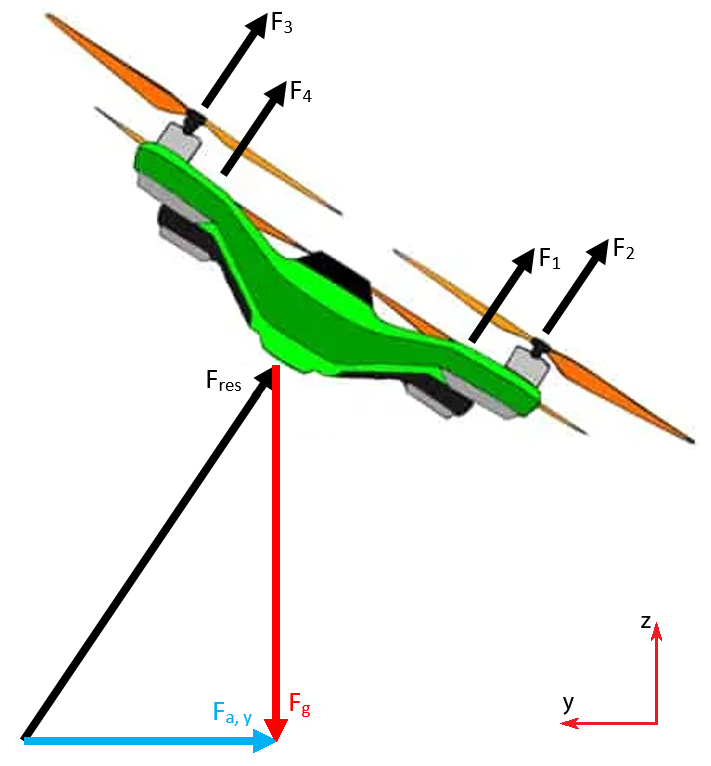
\includegraphics[width=12cm]{Pictures/Forces_Rolled.png}}
\caption{wirkende Kräfte für gerollten \Quad\ \comp{Quad1}}
\label{fig:ForcesRolled}
\end{center}

\vspace{0.25cm}
\refImgShort{fig:ForcesRolled} zeigt die auf einen \Quad\ wirkenden Kräfte, wenn sich dieser in einer gerollten Orientierung befindet. Hier entspricht der Betrag der Kraft entlang der z-Achse der Gewichtskraft.\\
Die Kraft $F_{res}$ wird mit der Gewichtskraft $F_g$ überlagert. Die hieraus resultierende Kraft kann in drei Kräfte aufgeteilt werden, welche parallel zu den kartesischen Achsen angeordnet sind. Hieraus berechnet sich die Beschleunigung, welche auf den \Quad\ wirkt.
\end{figure}




\newSec{Pose}{2}
Eine Pose ist die Positions- und Lagebeschreibung in einem Raum. \missing[quelle]










\newSec{lokale Pose}{3}
\missing



\newSec{globale Pose}{3}
\missing










